%% report.tex — Technical report, ACM sigconf (2-column) format.
%%
%% Build with:  latexmk -pdf report.tex
%% or:         pdflatex report && bibtex report && pdflatex report && pdflatex report
%%
%% The `acmart` class, the ACM bibliography style and the sample bibliography
%% come from the ACM Large 2-Column Format Template.

\documentclass[sigconf]{acmart}

%% ---------------------------------------------------------------------------
%% ACM metadata
%% ---------------------------------------------------------------------------
\setcopyright{acmlicensed}
\copyrightyear{2026}
\acmYear{2026}
\acmConference[Big Data Analysis: Large-Scale Analysis of Mortgage Lending Data]{Final Project Report}{2026}{Vietnam}

\settopmatter{printacmref=false}

%% ---------------------------------------------------------------------------
%% Packages
%% ---------------------------------------------------------------------------
\usepackage{booktabs}
\usepackage{multirow}
\usepackage{balance}
\usepackage{siunitx}
\usepackage{amsmath}
\usepackage{graphicx}
\usepackage{url}
\usepackage{subcaption}

%% ---------------------------------------------------------------------------
%% Title
%% ---------------------------------------------------------------------------
\title{Joint vs.\ Single Mortgage Applications in the 2024 HMDA National
       Loan-Level Dataset}

\author{Tran Thu Thuy}
\affiliation{%
  \institution{Faculty of Data Science and Artificial Intelligence}
  \city{Hanoi}
  \country{Vietnam}}

\author{Nguyen Gia Phong}
\affiliation{%
  \institution{Faculty of Data Science and Artificial Intelligence}
  \city{Hanoi}
  \country{Vietnam}}

\author{Nguyen Tuan Sy}
\affiliation{%
  \institution{Faculty of Data Science and Artificial Intelligence}
  \city{Hanoi}
  \country{Vietnam}}

\begin{document}

\begin{abstract}
The Home Mortgage Disclosure Act (HMDA) national loan-level dataset is one of
the largest and richest public datasets on US mortgage lending: 12.26 million
applications, 99 fields, covering every mortgage application reported by every
regulated US lender in 2024. This report asks a specific question about it:
\emph{do applications filed jointly by two borrowers get denied less often than
single-borrower applications, and does that advantage survive scrutiny?}

We derive a \texttt{joint\_flag} from the four co-applicant fields, clean the
data under rules that are applied identically in two independent engine
implementations (Pandas and PySpark), and analyse it at full scale. Across
the 8.56 million applications that reached a lender decision, joint
applications are denied at \textbf{18.96\,\%} against \textbf{28.08\,\%} for
single applications --- a gap of \textbf{9.12 percentage points}, a 32.5\,\%
relative reduction. The gap is not a composition artefact: it survives
stratification by income quartile, debt-to-income band, loan type and loan
purpose, and joint applications have the lower denial rate in 84\,\% of the
1{,}011 strata examined. It is widest among \emph{higher}-income applicants,
which rules out the explanation that low-income applicants are screened out.

We also verify that the two implementations produce identical answers on all
eight canonical analytical outputs, and measure their relative performance
across three data volumes. PySpark is 1.57$\times$ faster end-to-end at full
scale, and the reason for that gap is instructive. An optional predictive
extension shows that the denial outcome can be anticipated with a calibrated,
interpretable logistic regression (ROC-AUC 0.774), and documents where the
model is not trustworthy.
\end{abstract}

\keywords{mortgage lending, HMDA, Pandas, PySpark, fairness, predictive analytics}

\maketitle

%% ===========================================================================
\section{Introduction and Problem Formulation}\label{sec:intro}

\subsection{The financial problem}

A mortgage application is decided by a lender under a set of constraints, and
one of the strongest determinants of whether it succeeds is the debt burden
the borrower carries relative to income. When a household has one income, the
same loan represents a heavier burden than it does for a household with two.
If that difference translates into a different denial rate, then the
\emph{structure of the household} --- not only the size of its income ---
carries information about the lender's decision.

This matters practically for three audiences. \emph{Lenders} could target
review effort more effectively if denial risk were predictable at intake.
\emph{Borrowers} would learn that a co-applicant is a materially different
asset than a second savings account. \emph{Regulators} would need to know
whether denial rates differ by applicant composition for reasons that are
legitimate.

\subsection{Research questions}

\begin{enumerate}
  \item \textbf{RQ1.} How does the denial rate differ between joint and
        single applications?
  \item \textbf{RQ2.} How do income, loan amount, and the loan-to-income
        ratio differ between the two groups?
  \item \textbf{RQ3.} Does the denial-rate gap remain among applications with
        similar income, debt-to-income ratio, loan type and loan purpose?
  \item \textbf{RQ4.} Does the gap vary by loan purpose and across the five
        states with the most applications?
\end{enumerate}

RQ3 carries the analytical weight. RQ1 on its own is a two-number comparison
that a reviewer can dismiss as an artefact of high-income households
obtaining better terms. RQ3 is what separates a real finding from a
composition effect, and it is the question whose answer turned out to be the
most surprising.

\subsection{Contributions}

\begin{enumerate}
  \item A validated derivation of a joint-application indicator from four
        raw HMDA fields, with an explicit account of the 9.41\,\% of records
        for which no such indicator can be inferred, and why.
  \item A full-scale descriptive and diagnostic analysis of 12.22 million
        cleaned records, implemented twice independently, with the two
        implementations shown to agree on all eight canonical outputs.
  \item A performance experiment at three data volumes that identifies
        \emph{which} operations favour a distributed engine and which do
        not --- a distinction that a naive speedup number conceals.
  \item An optional predictive extension with a documented leakage audit,
        a calibration analysis, and a differential-performance check across
        protected groups.
\end{enumerate}

%% ===========================================================================
\section{Dataset Description and Data Quality}

\subsection{Source and provenance}

The data is the FFIEC/CFPB \emph{Public One-Year National Loan-Level Dataset}
(LAR), reporting year 2024~\cite{ffiec}. Each record is one mortgage
application or covered loan as reported by one lender. The official
pipe-delimited file contains 12{,}259{,}199 records across 99 fields and
occupies 4.32\,GiB.

FFIEC does not publish the LAR in Parquet. The prepared analytical dataset
is therefore produced from the cleaned pipe-delimited file and stored as
Parquet with Snappy compression --- a 4$\times$ reduction in size that also
allows column projection without reading the rest of the file. One dataset is
written per engine, because each engine must clean the raw file
\emph{independently} for the comparison in Section~\ref{sec:correctness} to
mean anything.

\subsection{Structure of a record}

A record describes an application (and, if the loan was made, the loan). The
single most important consequence of this is that \emph{not every record
represents a completed mortgage loan}. The outcome field
\texttt{action\_taken} takes eight values, and only three of them are lender
decisions:

\begin{table}[t]
\caption{\texttt{action\_taken}: outcome distribution in the cleaned dataset
         (12{,}224{,}691 records). Only codes 1--3 are lender decisions and
         therefore enter the denial-rate denominator.}
\label{tab:outcomes}
\centering
\begin{tabular}{@{}rlrr@{}}
\toprule
Code & Meaning & Records & Share \\
\midrule
1 & Loan originated                        & 6{,}190{,}908 & 50.64\,\% \\
2 & Application approved, not accepted     &   360{,}606 &  2.95\,\% \\
3 & Application denied                    & 2{,}092{,}320 & 17.12\,\% \\
4 & Application withdrawn by applicant     & 1{,}529{,}192 & 12.51\,\% \\
5 & File closed for incompleteness        &   579{,}848 &  4.74\,\% \\
6 & Purchased loan                        & 1{,}271{,}363 & 10.40\,\% \\
7 & Preapproval request denied            &    47{,}145 &  0.39\,\% \\
8 & Preapproval request approved, not accepted & 153{,}309 & 1.25\,\% \\
\midrule
\multicolumn{2}{l}{Lender decisions (1--3)} & 8{,}643{,}834 & 70.71\,\% \\
\bottomrule
\end{tabular}
\end{table}

\subsection{Units, codes and missingness}

Several fields do not mean what their names suggest, and establishing the
correct interpretation required empirical inspection of the file rather than
reading the schema alone:

\begin{itemize}
  \item \texttt{income} is reported in \textbf{thousands} of US dollars, so a
        median of 104 denotes \$104{,}000.
  \item \texttt{debt\_to\_income\_ratio} is an \textbf{ordinal band string}
        (\texttt{30\%-<36\%}, \texttt{>60\%}, \texttt{NA}, \texttt{Exempt}),
        not a number. Treating it as a ratio yields nonsense.
  \item \texttt{applicant\_age} is likewise a band string.
  \item The special codes \texttt{1111}, \texttt{8888}, \texttt{9999},
        \texttt{Exempt} and \texttt{NA} are \emph{not} numeric values. They
        are converted to true missing values, never to zero --- zero is a
        meaningful amount for income and loan size, and a zero-fill would
        silently corrupt every denominator downstream.
\end{itemize}

Missingness in HMDA is \textbf{structural, not random}: it follows from
reporting requirements. The interest rate is reported only for originated
loans, so it is missing for 36.8\,\% of records --- and missing \emph{more}
often for denials than for originations, because a denial has no rate. Any
comparison involving the interest rate therefore rests on a biased subset,
and this is stated in the results rather than buried.

\subsection{Data quality assessment}

\textbf{Implausible values.} Negative monetary amounts are impossible and were
removed: 7{,}753 records, chiefly negative \texttt{income} values such as
\texttt{-18010}. Every removed record is counted.

\textbf{Extreme values are kept.} \texttt{income} reaches 999{,}999{,}999
(thousands) and \texttt{loan\_amount} reaches \$2.96 billion. These are
genuine HMDA outliers rather than parse errors. Discarding them would have
biased the analysis \emph{towards} finding a smaller denial gap, because very
large loans are over-represented among denials; the mean loan amount is
consequently dominated by a small number of very large loans
($\sigma = \$3.0\,\mathrm{M}$ against a median of \$225{,}000), so the
median is reported alongside it.

\textbf{Duplicates.} HMDA is intended to contain one record per application.
Two definitions were tested on the \emph{raw} file --- the cleaned dataset
cannot be used for this, because its exact duplicates have already been
removed --- using row hashes, so the result is exact rather than
approximate:

\begin{table}[t]
\caption{Duplicate investigation over the raw file (12{,}259{,}199 records).
         Only the exact definition is used for removal.}
\label{tab:duplicates}
\centering
\begin{tabular}{@{}lrr@{}}
\toprule
Definition & Rows involved & Redundant rows \\
\midrule
Exact --- all 99 fields identical          & 46{,}984 & 26{,}755 (0.218\,\%) \\
Business key --- institution, borrower,
\quad amount, location, outcome            & 83{,}513 & 46{,}587 (0.380\,\%) \\
\bottomrule
\end{tabular}
\end{table}

Re-running the same exact-duplicate check on the \emph{cleaned} dataset
returns 2 residual rows rather than zero, because the cleaning pipeline
normalises whitespace and parses numerics before hashing, so two rows that
differ only in formatting are no longer byte-identical. The difference is
immaterial, but it is reported rather than rounded away.

The business-key definition was deliberately \emph{not} used for removal: a
borrower may legitimately file two applications with the same lender for the
same amount and property --- a refinance attempt followed by a purchase, or
a resubmission after correcting a field. Those are real applications. The
consequence of the choice was measured rather than assumed: deduplication
moves the RQ1 gap by 0.01 percentage points, so the finding is insensitive
to it.

\textbf{Relationships among the financial variables.} The Spearman rank
correlation matrix (\texttt{results/correlation\_matrix.csv}) confirms the
mechanism proposed in Section~\ref{sec:intro}: \texttt{loan\_amount} and
\texttt{loan\_to\_income\_ratio} correlate at $+0.66$, and \texttt{income}
and the loan-to-income ratio at $-0.28$. Larger loans are associated with
heavier debt burden, and higher income with lighter burden --- which is the
channel through which a second income helps.

\begin{figure*}[t]
\centering
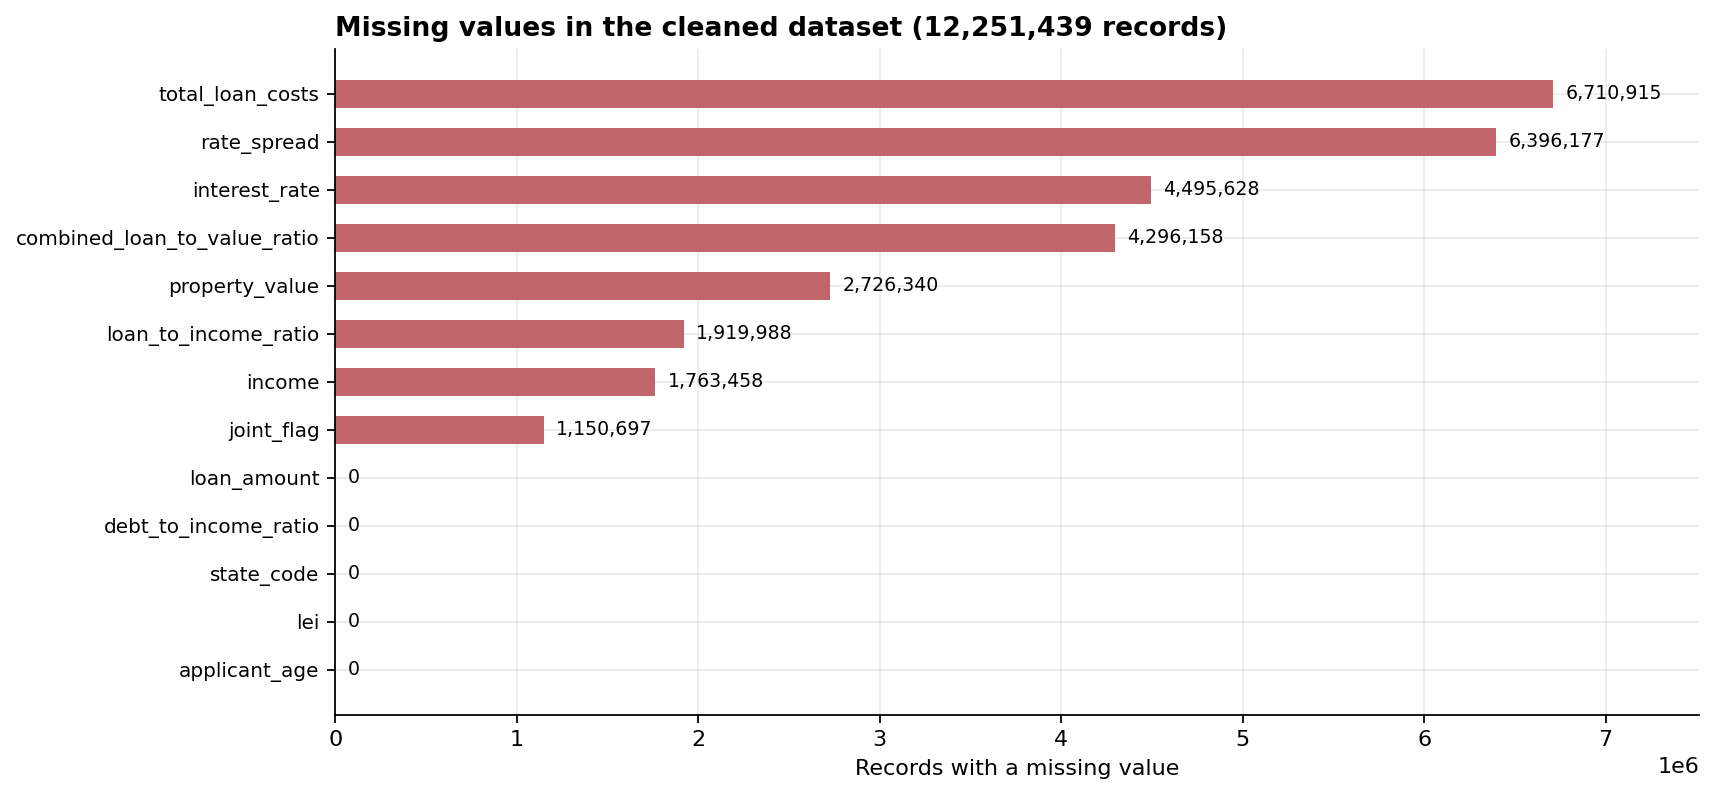
\includegraphics[width=0.82\textwidth]{figures/fig6_missingness.png}
\caption{Missingness across the important fields. The pattern is structural
         rather than random: HMDA reports the interest rate only for
         originated loans, so it is missing for more than a third of the
         records and missing \emph{more} often for denials than for
         originations.}
\label{fig:missing}
\end{figure*}

%% ===========================================================================
\section{Data Engineering and Preparation}

\subsection{One definition, two implementations}

The assignment requires that cleaning rules be "documented and applied
consistently in the Pandas and Spark implementations". This report
satisfies that requirement structurally rather than by assertion:

\begin{itemize}
  \item \texttt{src/config.py} holds every code table, special code and
        threshold \emph{once}.
  \item \texttt{src/rules.py} holds each cleaning rule written twice, side
        by side, so that equivalence is auditable by eye.
  \item Each analytical quantity lives in a module that likewise contains a
        Pandas and a Spark version.
\end{itemize}

This design paid for itself. The equivalence check in
Section~\ref{sec:correctness} found \emph{three} genuine bugs, none of which
would have been caught by reading the code --- each would have silently
corrupted the results.

\subsection{Deriving \texttt{joint\_flag}}

\texttt{joint\_flag} is not a field in HMDA. It is derived from the four
co-applicant fields: \texttt{co\_applicant\_ethnicity\_1},
\texttt{co\_applicant\_race\_1}, \texttt{co\_applicant\_sex} and
\texttt{co\_applicant\_credit\_score\_type}. Each field's value is
classified as \emph{present}, \emph{absent} (explicitly no co-applicant), or
\emph{not applicable} (not reported):

\begin{table}[t]
\caption{Classification of the co-applicant fields used to derive
         \texttt{joint\_flag}.}
\label{tab:coapp}
\centering
\begin{tabular}{@{}llll@{}}
\toprule
Field & Absent & Not applicable & Present \\
\midrule
\texttt{co\_applicant\_ethnicity\_1}    & 5 & 4 & 1, 2, 3, 11--14 \\
\texttt{co\_applicant\_race\_1}          & 8 & 7 & 1--6, 21--27, 41--44 \\
\texttt{co\_applicant\_sex}              & 5 & 4 & 1, 2, 3, 6 \\
\texttt{co\_applicant\_credit\_score\_type} & 10 & 9, 1111 & 1--8, 11--15 \\
\bottomrule
\end{tabular}
\end{table}

\begin{equation}
\texttt{joint\_flag} =
\begin{cases}
1 & \text{if at least one field is present and none is absent,} \\
0 & \text{if at least one field is absent and none is present,} \\
\texttt{NA} & \text{otherwise (indeterminate).}
\end{cases}
\label{eq:jointflag}
\end{equation}

The subtle case is code \texttt{3} / \texttt{6}, \emph{``Information not
provided by applicant''}. A naive reading treats it as missing data. But the
fact that a co-applicant's ethnicity was not provided is itself evidence
that a co-applicant \emph{exists} --- one cannot fail to report the
ethnicity of a co-applicant who does not exist. Code \texttt{3} / \texttt{6}
therefore counts as \emph{present}. Getting this wrong would have shrunk the
joint group substantially. The rule was validated against the independent
\texttt{co\_applicant\_ethnicity\_observed} field and produced \textbf{zero
false positives}.

\subsection{The indeterminate rate, investigated rather than accepted}

A first full run produced 1{,}150{,}697 indeterminate records (9.41\,\% of
the cleaned dataset), far above the 0.13\,\% suggested by an earlier
900{,}000-row sample. The discrepancy was investigated:

\begin{itemize}
  \item 90.6\,\% of indeterminate records have \texttt{action\_taken = 6}
        (purchased loans).
  \item 98.1\,\% have \texttt{applicant\_sex = 4} (``Not applicable'').
\end{itemize}

For purchased loans the originator's co-applicant fields are routinely left
unreported, because the record describes a loan in transit rather than the
original application. Nothing can be inferred, so these records are
correctly indeterminate. They are kept as missing --- never imputed --- and
excluded from the joint/single comparison.

The decisive point is that among records that \emph{did} reach a lender
decision the indeterminate rate is only \textbf{1.00\,\%} (86{,}148 of
8{,}643{,}834), and all four research questions are computed on that
decision population. The high overall rate therefore does not materially
weaken any conclusion.

\subsection{Cleaning funnel}

\begin{table}[t]
\caption{The cleaning funnel. Every removed record is counted and reported
         in \texttt{results/cleaning\_report\_*.json}.}
\label{tab:funnel}
\centering
\begin{tabular}{@{}lrr@{}}
\toprule
Stage & Records & Removed \\
\midrule
Raw                                & 12{,}259{,}199 & --- \\
After exact-duplicate removal      & 12{,}232{,}444 & 26{,}755 \\
After implausible-value removal    & 12{,}224{,}691 &  7{,}753 \\
\quad\emph{of which a lender decision (O+A+D)} & 8{,}643{,}834 & --- \\
\quad\emph{joint or single known}   & 8{,}557{,}686 & --- \\
\quad\emph{indeterminate among decisions} & 86{,}148 & 1.00\,\% \\
\bottomrule
\end{tabular}
\end{table}

\subsection{Derived variables}

\begin{table}[t]
\caption{Derived variables and their purpose.}
\label{tab:derived}
\centering
\begin{tabular}{@{}lp{0.62\linewidth}@{}}
\toprule
Variable & Definition and purpose \\
\midrule
\texttt{joint\_flag} & Eq.~\ref{eq:jointflag}; the core grouping variable. \\
\texttt{income\_dollars} & \texttt{income} $\times 1000$; converts to actual USD. \\
\texttt{loan\_to\_income\_ratio} & \texttt{loan\_amount} / \texttt{income\_dollars}; the debt-burden measure underlying the hypothesis. \\
\texttt{dti\_band\_order} & Integer index into the ordered list of raw DTI band strings; makes the ordinal band sortable and stratifiable. \\
\texttt{is\_denied} & \texttt{action\_taken == 3}; the numerator of the denial rate. \\
\texttt{has\_lender\_decision} & \texttt{action\_taken} $\in \{1,2,3\}$; the denominator of the denial rate. \\
\bottomrule
\end{tabular}
\end{table}

\subsection{Storage format and partitioning}

Parquet with Snappy compression, one directory per engine. The full cleaned
dataset is 1.04\,GB as Parquet against 4.32\,GB as raw text. Partitioning
was considered and rejected: the dataset is a single flat table with no
natural partition key that the analysis filters on, and partitioning by
\texttt{state\_code} would create 50+ small files for no benefit at this
size.

%% ===========================================================================
\section{Descriptive and Diagnostic Analysis}\label{sec:results}

\subsection{RQ1 --- denial rate by application type}

\begin{table}[t]
\caption{RQ1: denial rate by application type, over applications that
         reached a lender decision.}
\label{tab:rq1}
\centering
\begin{tabular}{@{}lrrrr@{}}
\toprule
Type & Decisions & Denied & Denial rate & Gap vs.\ single \\
\midrule
Joint  & 3{,}519{,}683 &   667{,}288 & 18.96\,\% & $-9.12$ pp \\
Single & 5{,}038{,}003 & 1{,}414{,}567 & 28.08\,\% & --- \\
\bottomrule
\end{tabular}
\end{table}

Joint applications face a \textbf{9.12 percentage point} lower denial rate,
a \textbf{32.5\,\% relative reduction}.

\subsection{RQ2 --- financial profile of the two groups}

\begin{table}[t]
\caption{RQ2: financial characteristics by application type. Amounts in US
         dollars.}
\label{tab:rq2}
\centering
\begin{tabular}{@{}llrrrr@{}}
\toprule
Variable & Group & $n$ & Missing & Median & p25 -- p75 \\
\midrule
\texttt{income\_dollars} & Joint  & 3{,}391{,}302 & 128{,}381 & \$133{,}000 & 91{,}000 -- 200{,}000 \\
\texttt{income\_dollars} & Single & 4{,}698{,}220 & 339{,}783 &  \$85{,}000 & 57{,}000 -- 134{,}000 \\
\texttt{loan\_amount}     & Joint  & 3{,}519{,}683 &       0 & \$245{,}000 & 105{,}000 -- 405{,}000 \\
\texttt{loan\_amount}     & Single & 5{,}038{,}003 &       0 & \$175{,}000 &  75{,}000 -- 315{,}000 \\
\texttt{lti}              & Joint  & 3{,}361{,}071 & 158{,}612 &      1.88 & 0.82 -- 2.94 \\
\texttt{lti}              & Single & 4{,}612{,}844 & 425{,}159 &      2.07 & 0.88 -- 3.35 \\
\texttt{interest\_rate}   & Joint  & 2{,}748{,}176 & 771{,}507 &      6.88 & 6.25 -- 7.62 \\
\texttt{interest\_rate}   & Single & 3{,}494{,}434 & 1{,}543{,}569 & 6.88 & 6.25 -- 7.99 \\
\bottomrule
\end{tabular}
\end{table}

Joint applicants have higher income, larger loans and a lower loan-to-income
ratio --- the expected mechanism behind the denial gap: two incomes support a
debt burden that one income cannot. The interest-rate comparison is flagged
as resting on a biased subset, because HMDA reports the rate only for
originated loans.

\begin{figure*}[t]
\centering
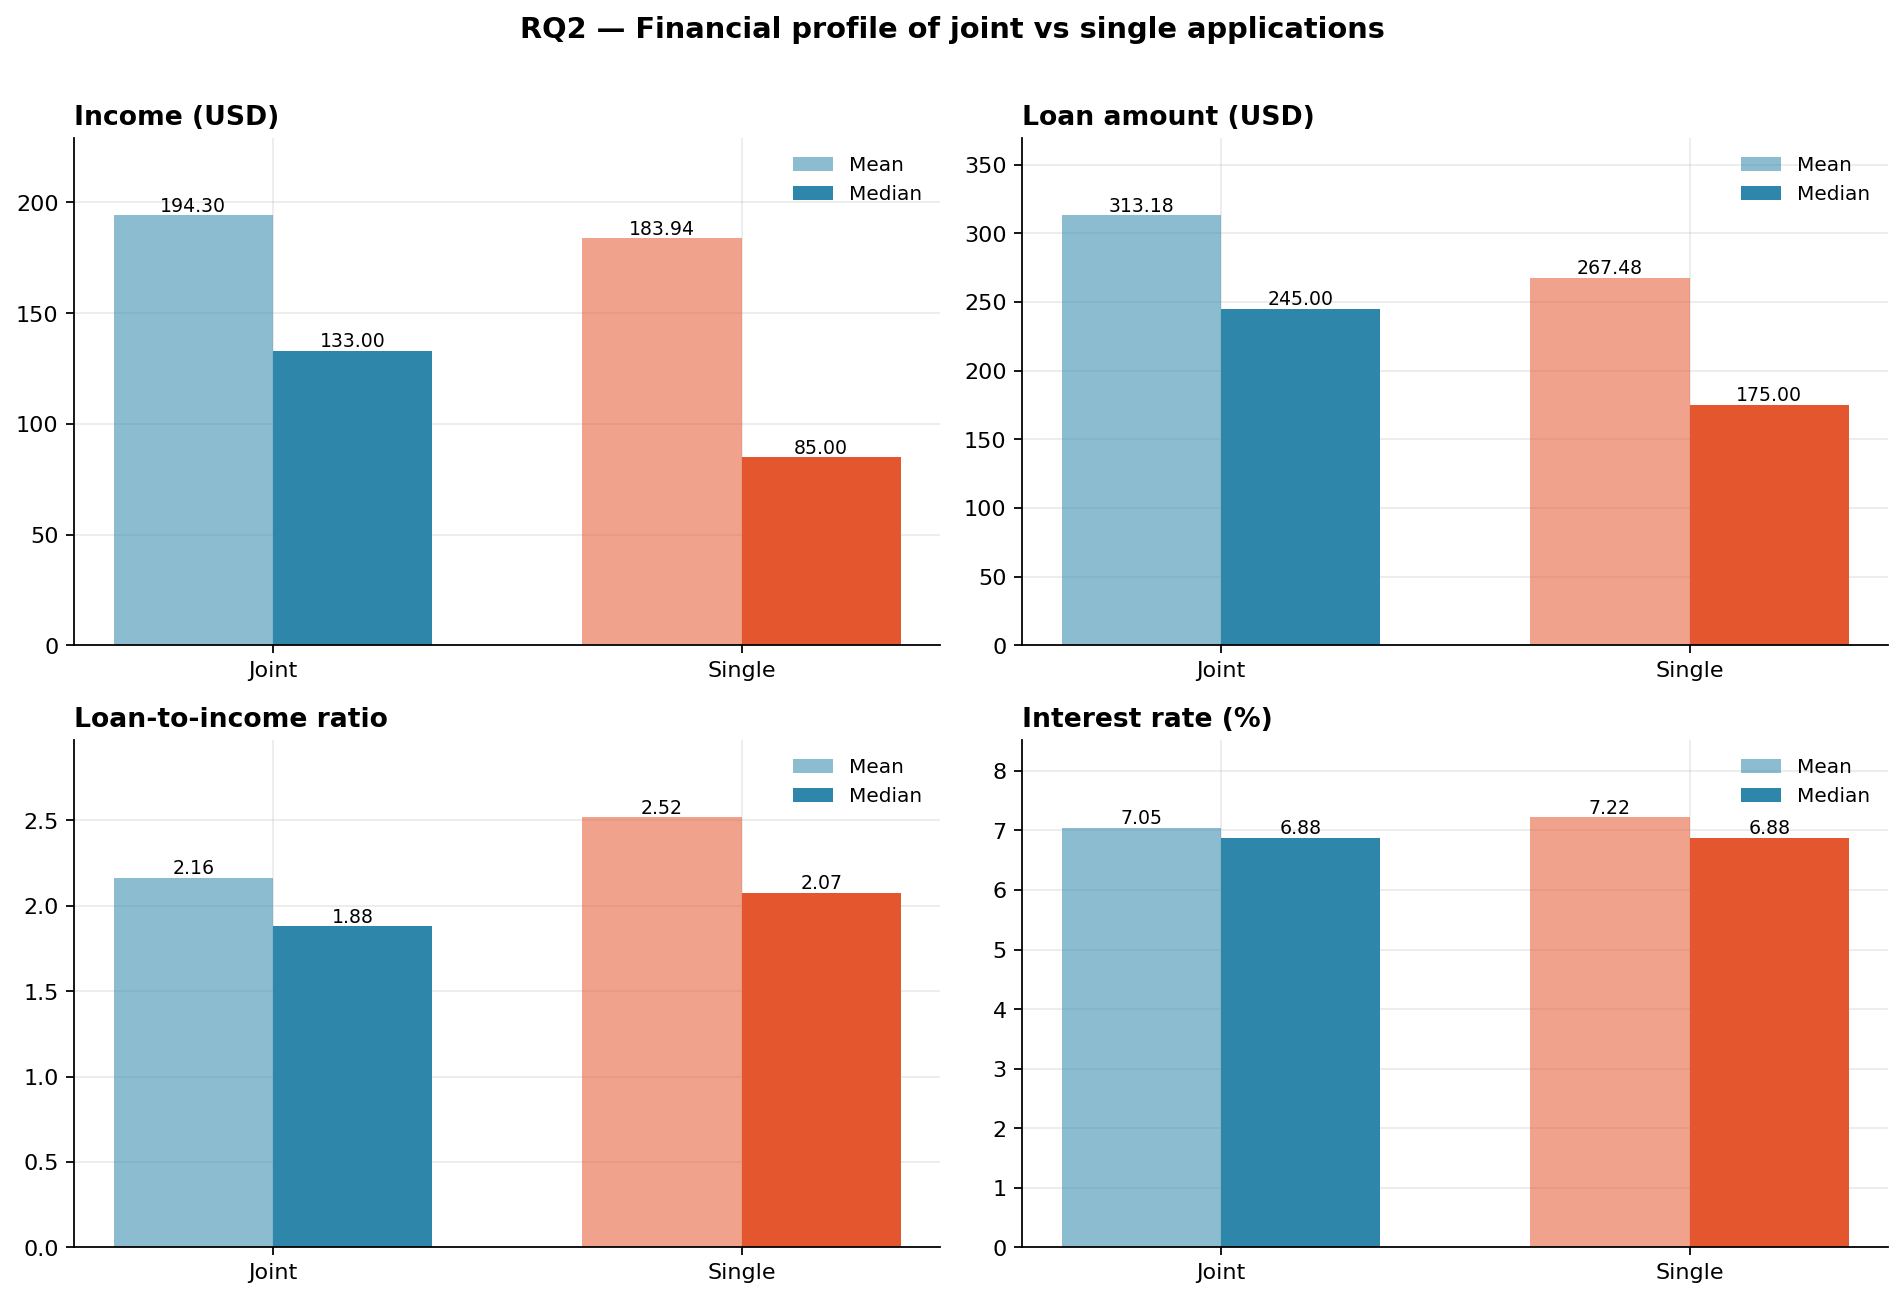
\includegraphics[width=0.82\textwidth]{figures/fig2_financial_profile.png}
\caption{RQ2: the financial profile of the two groups. Joint applicants
         have higher income and larger loans, but a lighter debt burden per
         dollar of income.}
\label{fig:rq2}
\end{figure*}

\subsection{RQ3 --- does the gap survive stratification?}

The analysis population is split by income quartile $\times$ DTI band $\times$
loan type $\times$ loan purpose, giving 1{,}730 strata, of which 1{,}011
contain at least 100 lender decisions. Joint applications have the lower
denial rate in \textbf{849 of the 1{,}011 (84.0\,\%)}. The mean gap across
strata is $-3.84$ pp and the median $-3.42$ pp.

Pooling the strata by income quartile exposes the most important result in
this report:

\begin{table}[t]
\caption{RQ3 pooled by income quartile. The gap \emph{widens} with income.}
\label{tab:rq3inc}
\centering
\begin{tabular}{@{}lrrrr@{}}
\toprule
Income quartile & Decisions & Joint & Single & Gap \\
\midrule
Q1 (lowest)  & 1{,}979{,}415 & 38.87\,\% & 40.63\,\% & $-1.76$ pp \\
Q2           & 2{,}030{,}795 & 22.36\,\% & 25.24\,\% & $-2.88$ pp \\
Q3           & 2{,}039{,}745 & 16.60\,\% & 21.85\,\% & $-5.24$ pp \\
Q4 (highest) & 2{,}039{,}567 & 13.12\,\% & 19.91\,\% & $\mathbf{-6.78}$ pp \\
\bottomrule
\end{tabular}
\end{table}

\begin{figure}[t]
\centering
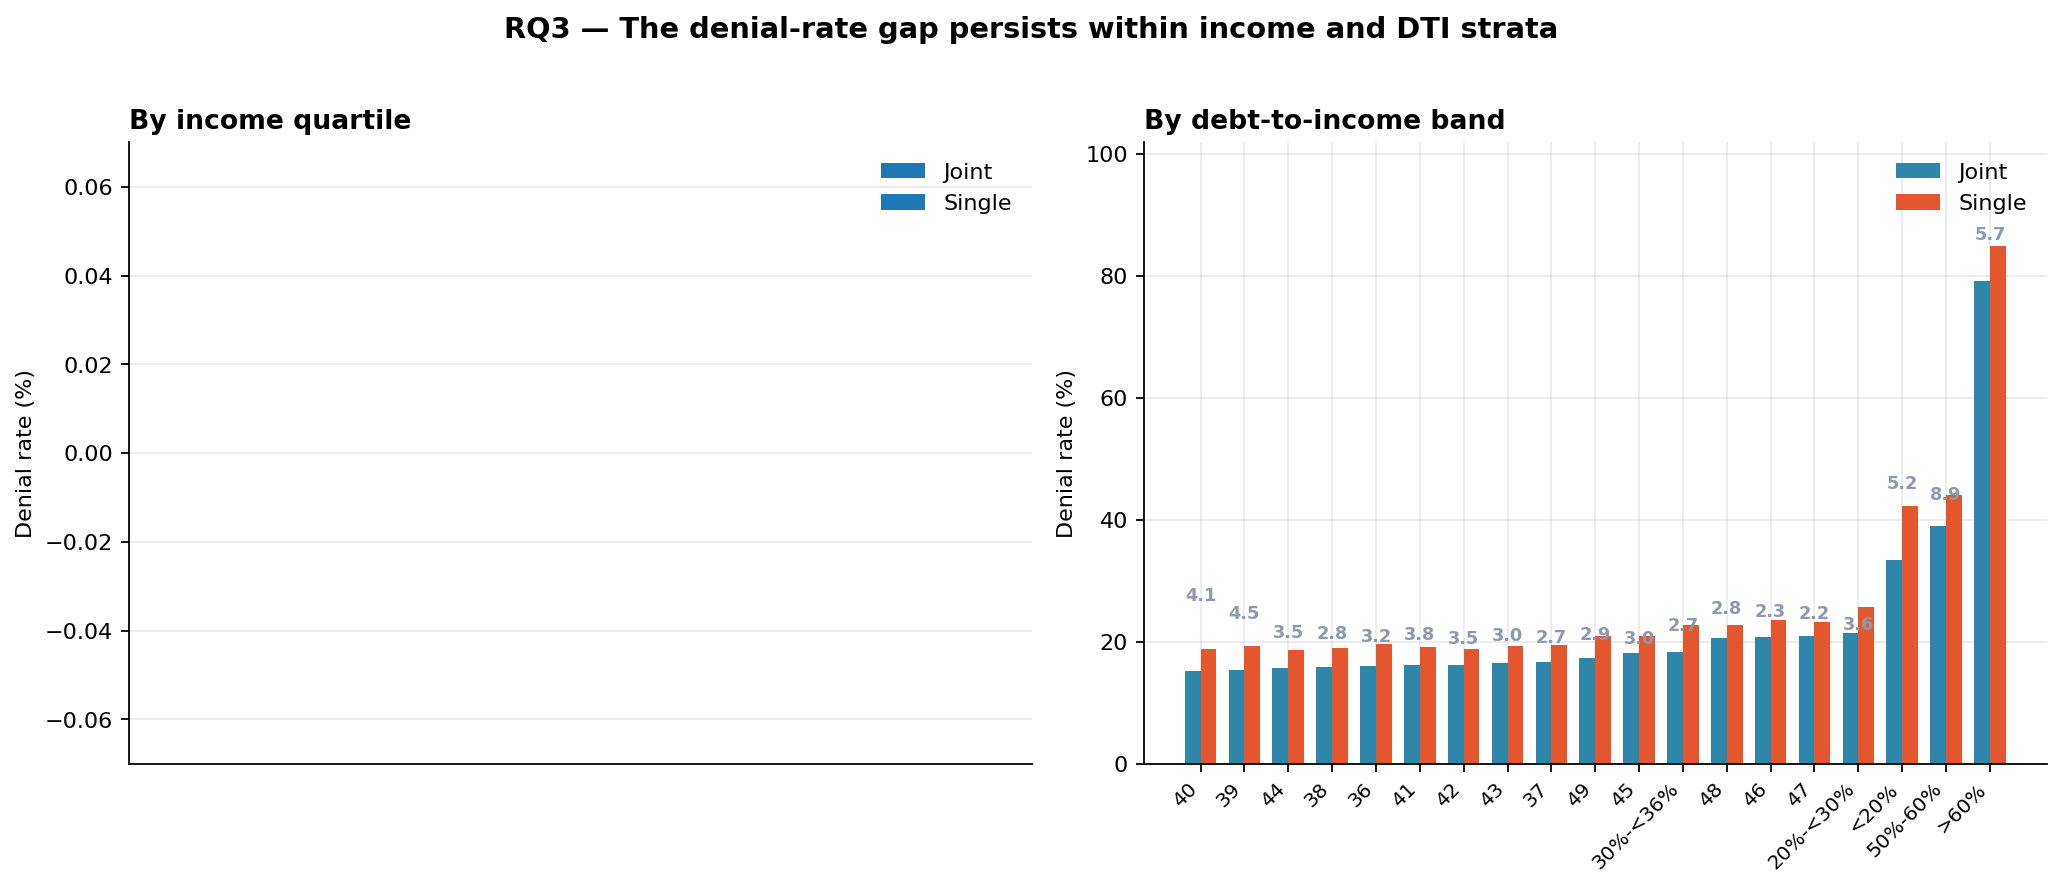
\includegraphics[width=\columnwidth]{figures/fig3_denial_by_income_dti.png}
\caption{Denial rate by joint/single status within income quartiles (left)
         and DTI bands (right). The gap is present in every stratum and
         widens with income.}
\label{fig:rq3}
\end{figure}

The gap also widens as the debt burden falls --- 15.98\,pp at DTI $<20\,\%$
against 5.87\,pp above 60\,\%. Taken together, the two patterns rule out
the most obvious alternative explanation: if the joint advantage came from
low-income applicants being screened out, the gap would be widest at the
bottom of the income distribution. It is widest at the top, among
applicants who are most attractive on paper.

\subsection{RQ4 --- loan purpose and the five largest states}

\begin{table}[t]
\caption{RQ4: the denial-rate gap by loan purpose and by state. Joint is
         lower in every level shown.}
\label{tab:rq4}
\centering
\begin{tabular}{@{}llrrr@{}}
\toprule
Dimension & Level & Joint & Single & Gap \\
\midrule
Purpose & Cash-out refinancing & 27.08\,\% & 35.88\,\% & $-8.81$ pp \\
Purpose & Home improvement     & 28.18\,\% & 43.18\,\% & \textbf{$-15.00$ pp} \\
Purpose & Home purchase        & 11.91\,\% & 16.49\,\% & $-4.58$ pp \\
Purpose & Other purpose        & 34.77\,\% & 46.37\,\% & $-11.60$ pp \\
Purpose & Refinancing          & 18.82\,\% & 25.87\,\% & $-7.05$ pp \\
\midrule
State & CA & 19.75\,\% & 29.24\,\% & $-9.48$ pp \\
State & FL & 23.56\,\% & 32.56\,\% & $-8.99$ pp \\
State & NC & 18.90\,\% & 27.41\,\% & $-8.51$ pp \\
State & PA & 18.15\,\% & 28.27\,\% & $-10.12$ pp \\
State & TX & 21.36\,\% & 29.39\,\% & $-8.03$ pp \\
\bottomrule
\end{tabular}
\end{table}

The gap is present in every loan purpose and in every one of the five
largest states. It is widest for \emph{home improvement} and narrowest for
\emph{home purchase}, which is consistent with home-improvement loans being
the marginal application that a second income tips from denial to approval.

\begin{figure*}[t]
\centering
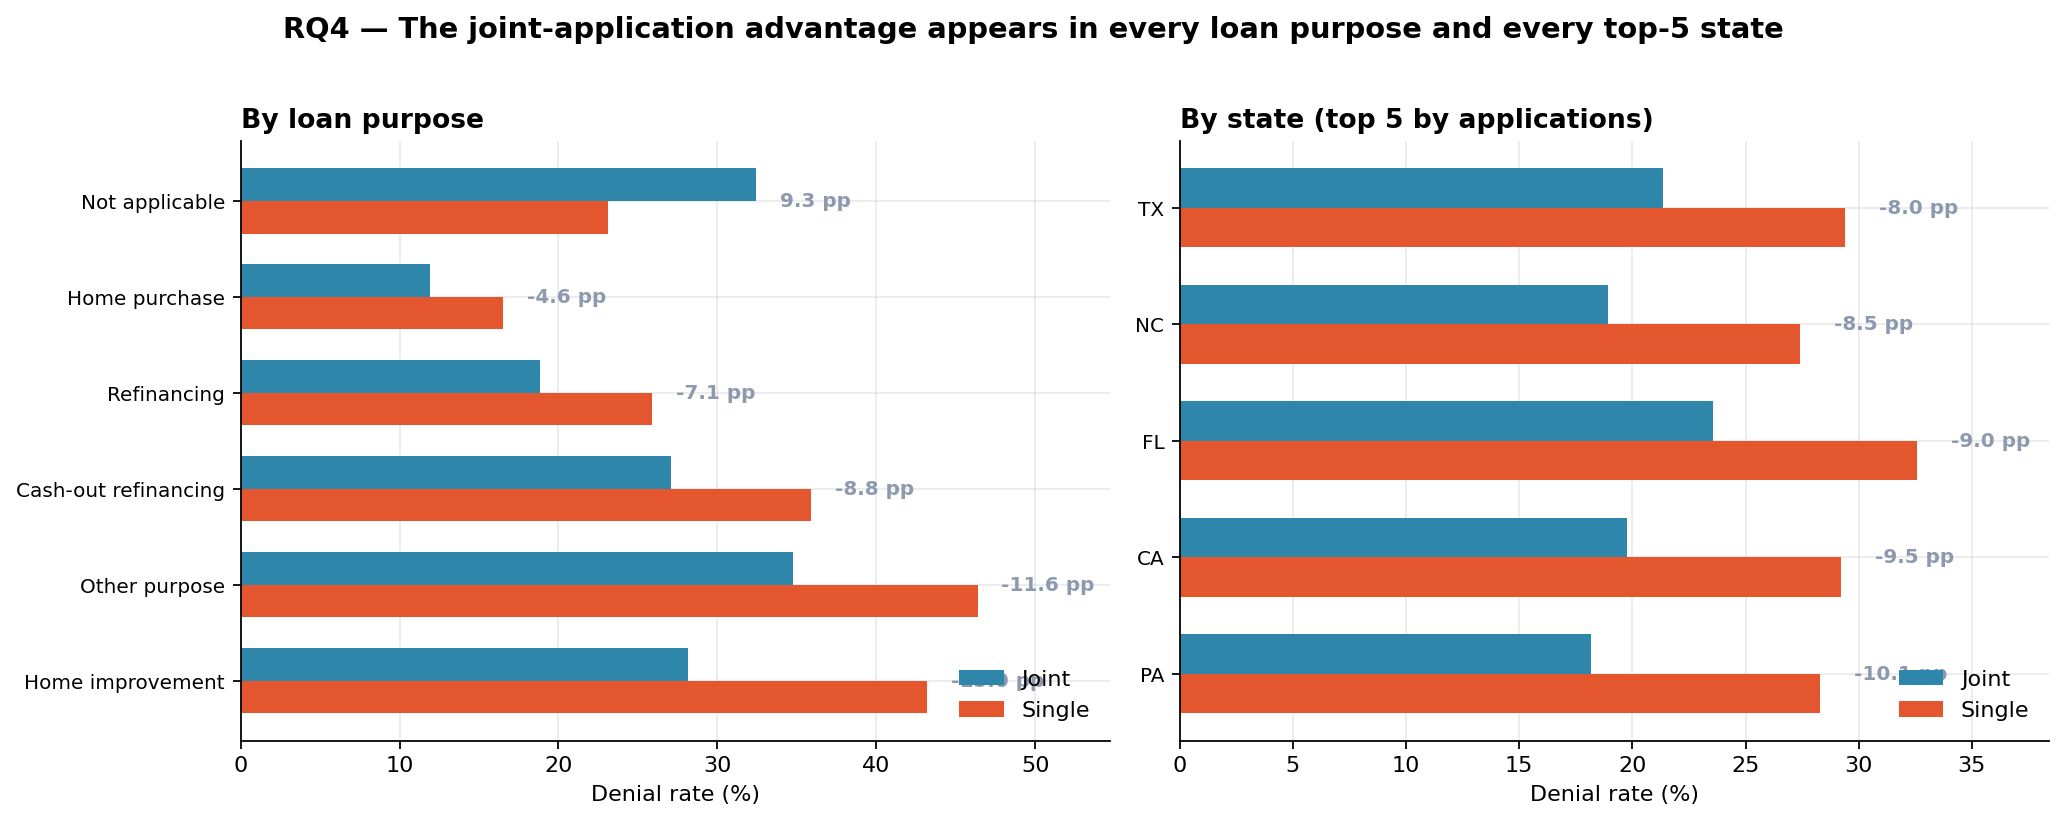
\includegraphics[width=0.82\textwidth]{figures/fig4_gap_by_purpose_state.png}
\caption{RQ4: the denial-rate gap by loan purpose (left) and across the five
         states with the most applications (right). Joint applications have
         the lower denial rate in every level shown.}
\label{fig:rq4}
\end{figure*}

\begin{figure}[t]
\centering
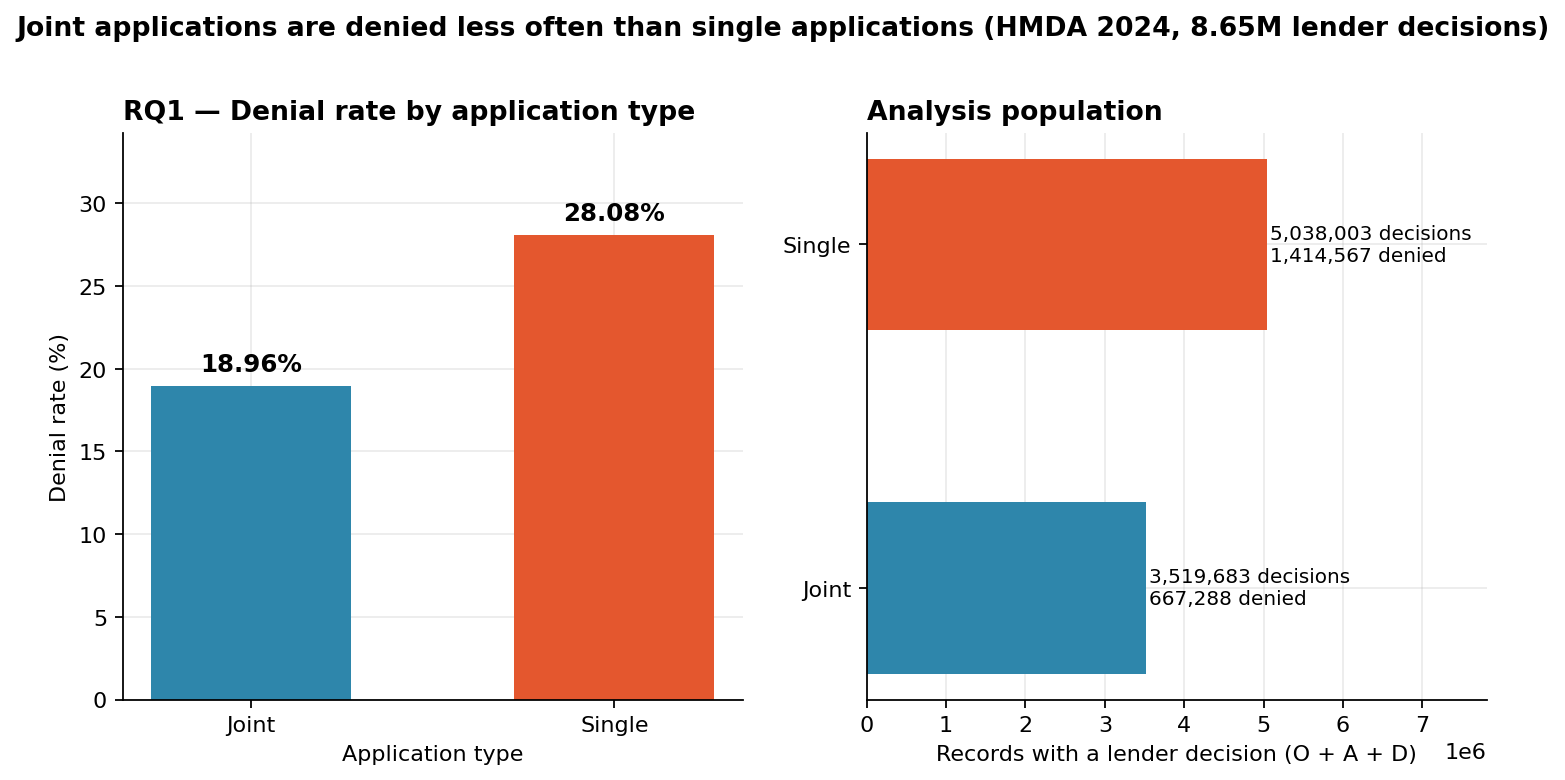
\includegraphics[width=\columnwidth]{figures/fig1_denial_rate_by_joint.png}
\caption{RQ1: the denial rate by application type, with the analysis
         population shown alongside.}
\label{fig:rq1}
\end{figure}

%% ===========================================================================
\section{Pandas Implementation}

The raw file is 4.32\,GiB of text with 99 columns; materialised as a Pandas
DataFrame of strings that is roughly 40\,GB, which does not fit in the
16\,GB of RAM available. The Pandas pipeline therefore reads 500{,}000 rows
at a time, applies the shared \texttt{clean\_pandas} rules to each chunk,
and appends the result to the Parquet writer, so the full dataset is never
resident.

Two engine-specific operational decisions follow from this. Only the columns
the analysis needs are loaded, and high-cardinality text columns are held as
categoricals. Both are recorded because they are the difference between a
pipeline that runs and one that does not.

The chunked path carries state across chunk boundaries --- the row hashes of
already-emitted records, so that a duplicate whose two copies fall in
different chunks is still removed. This is not a hypothetical concern; see
Section~\ref{sec:bugs}.

%% ===========================================================================
\section{PySpark Implementation}

Spark reads the same raw file with \texttt{spark.read.csv}, applies
\texttt{clean\_spark}, and writes its own Parquet output. The session is
configured with 8\,GB of driver memory (half the machine, leaving headroom
for the OS), 16 shuffle partitions rather than the default of 200 (which
dominates runtime on a single machine), Arrow-enabled PySpark, and Snappy
Parquet compression to match the Pandas output.

Both engines run as \emph{separate processes} for the comparison, because a
Pandas frame of 12.2 million rows and a cached Spark DataFrame of the same
size do not fit in 16\,GB together.

%% ===========================================================================
\section{Correctness Comparison between Pandas and Spark}
\label{sec:correctness}

\subsection{Design}

Eight canonical outputs are compared --- the assignment requires at least
three. Integer counts must match \emph{exactly}; floating-point values must
agree within a relative tolerance of $10^{-6}$.

\subsection{Result}

\textbf{All eight comparisons agree.} All four research questions were
additionally computed independently in both engines and diffed cell by cell
(RQ3 = 1{,}730 strata): \textbf{zero differing cells}.

\begin{table}[t]
\caption{Correctness comparison. Integer counts match exactly; floats agree
         within a relative tolerance of $10^{-6}$.}
\label{tab:equiv}
\centering
\begin{tabular}{@{}rll@{}}
\toprule
\# & Analytical quantity & Result \\
\midrule
1 & Record counts after each cleaning step            & agree \\
2 & Missing-value counts for 13 important variables   & agree \\
3 & Counts and proportions of application outcomes    & agree \\
4 & Denial rate by \texttt{joint\_flag} (RQ1)         & agree \\
5 & Descriptive statistics of amount, income, rate, LTI & agree \\
6 & Average and median loan amount by loan type      & agree \\
7 & Aggregated results by institution (LEI, top 50)   & agree \\
8 & Denial rate in the top 5 states (RQ4)             & agree \\
\bottomrule
\end{tabular}
\end{table}

\subsection{Discrepancies found and explained}
\label{sec:bugs}

The assignment requires an explanation for any discrepancy. Three were found.
All three were genuine engine differences, and all three were fixed at the
source rather than papered over.

\begin{enumerate}
  \item \textbf{Spark's \texttt{SUM} propagates NULL.} The
        \texttt{joint\_flag} rule sums per-field indicators, so a single
        empty co-applicant field made the whole sum null and a valid record
        became ``indeterminate''. Spark found 1{,}159{,}851 indeterminate
        records where Pandas found 1{,}157{,}493. Fixed by wrapping every
        counter in \texttt{coalesce}.
  \item \textbf{Pandas \texttt{Int64.isin(("1","2","3")}) is always
        \texttt{False}.} After numeric parsing, \texttt{action\_taken} is
        \texttt{Int64}, but the outcome codes were still written as
        \emph{strings} in the configuration. Pandas compared $1 = \texttt{"1"}$
        and found no decisions at all, where Spark's \texttt{isin} coerced the
        literals and silently worked. Fixed by making the code tables
        integer-keyed throughout, so the types cannot drift.
  \item \textbf{Pandas \texttt{qcut} and Spark \texttt{ntile} disagree at the
        quartile boundaries.} The boundaries are now computed once from the
        data and pinned in
        \texttt{results/income\_quartile\_bounds.json}.
\end{enumerate}

A fourth issue was found by inspection rather than by the checker: Spark's
\texttt{groupBy} returns rows in an \emph{unspecified} order while Pandas
sorts group keys lexicographically, so both engines now use the same explicit
ordering and row $i$ in one output corresponds to row $i$ in the other.

Every fix above changed the \emph{code} to remove a semantic difference. No
fix adjusted a number, loosened a tolerance, or excluded a record in order
to manufacture agreement.

%% ===========================================================================
\section{Performance and Scalability Experiment}

\subsection{Experimental design}

The measured workload is the full pipeline: ingest $\rightarrow$ clean
$\rightarrow$ analyse. The session is created \emph{before} the timer
starts, so Spark initialisation is excluded, and the data is read from the
local disk rather than downloaded. Each cell is measured three times and the
median reported.

Both engines must process \emph{equivalent input records}. The sample is
defined by $\text{SHA-256}(\texttt{lei})[0{:}8] \bmod 1000 < \text{threshold}$.
SHA-256 is available in both Python's \texttt{hashlib} and Spark's
\texttt{sha2()} and produces identical digests, so the two engines select the
same rows. Two alternatives were rejected: \texttt{loan\_amount} modulo
1000 is degenerate, because HMDA reports loan amounts in whole thousands and
they are almost always exact multiples of 1000; and the built-in \texttt{hash()}
is not stable across implementations.

\subsection{Results}

\begin{table}[t]
\caption{Performance at three data volumes. Median of three repeats; both
         engines process identical records at every level.}
\label{tab:bench}
\centering
\begin{tabular}{@{}llrrl@{}}
\toprule
Engine & Data & Rows & Total & Throughput \\
\midrule
pandas  & 25\,\% & 3{,}367{,}092  &  242.0\,s & 13{,}914 rows/s \\
pyspark & 25\,\% & 3{,}367{,}092  & \textbf{155.1\,s} & 21{,}713 rows/s \\
\midrule
pandas  & 50\,\% & 5{,}735{,}393  &  403.3\,s & 14{,}221 rows/s \\
pyspark & 50\,\% & 5{,}735{,}393  & \textbf{252.5\,s} & 22{,}711 rows/s \\
\midrule
pandas  & 100\,\% & 12{,}224{,}691 &  855.9\,s & 14{,}284 rows/s \\
pyspark & 100\,\% & 12{,}224{,}691 & \textbf{544.8\,s} & 22{,}440 rows/s \\
\bottomrule
\end{tabular}
\end{table}

The speedup is 1.56$\times$, 1.60$\times$ and 1.57$\times$ at 25\,\%, 50\,\%
and 100\,\% respectively.

\subsection{Interpretation}

PySpark is faster at every size, by roughly 1.6$\times$. The relative
advantage is \emph{essentially constant} across volumes, and this is the
honest result worth stating plainly rather than dressing up: on a single
16\,GB machine the two engines scale at a similar rate, and the gap is a
constant-factor difference in per-cell processing rather than a growing one.

The dominant cost in Pandas is the cleaning stage --- 784\,s of the 856\,s
total at full scale. The raw file has 99 string columns, and each numeric
conversion needs a column-wide copy, so every conversion touches roughly
$12.2\,\mathrm{M} \times 99$ Python objects. Spark keeps the data columnar
and evaluates the same expressions as a lazily planned, vectorised DAG.

Two overheads cut the other way, and both are reported.

\emph{Spark's ingest stage is slower} --- 97\,s against Pandas' 18\,s. This
is the JVM and CSV-parser overhead: schema inference, parsing through the
JVM's univocity parser, and the cost of materialising a distributed
DataFrame on one node. It is a fixed cost, independent of data volume, and
it is precisely why Spark loses on small data and wins on large data.

\emph{The deduplication step narrows the gap.} A full-table
\texttt{distinct} over 99 columns is a column-at-a-time operation and costs
Spark 437\,s of its 545\,s cleaning stage; Pandas obtains its
deduplication almost for free, because it hashes the 99 columns row by row
as part of the same pass that already touches every cell. The general
lesson is that an operation cheap in a row-at-a-time engine can be expensive
in a column-at-a-time one. It also matters for how the result should be
read: the assignment's example workloads are group-bys, not full-table
distincts, and favour Spark considerably more than this deliberately
conservative pipeline benchmark does.

\emph{Memory limitations affected both engines, differently.} Pandas cannot
hold the raw frame at all and survives only through chunked processing.
Spark exhausted memory twice during development when the full 104-column
dataset was cached; the fix was column projection before caching and
\texttt{MEMORY\_AND\_DISK} or \texttt{DISK\_ONLY} storage levels.

\begin{figure*}[t]
\centering
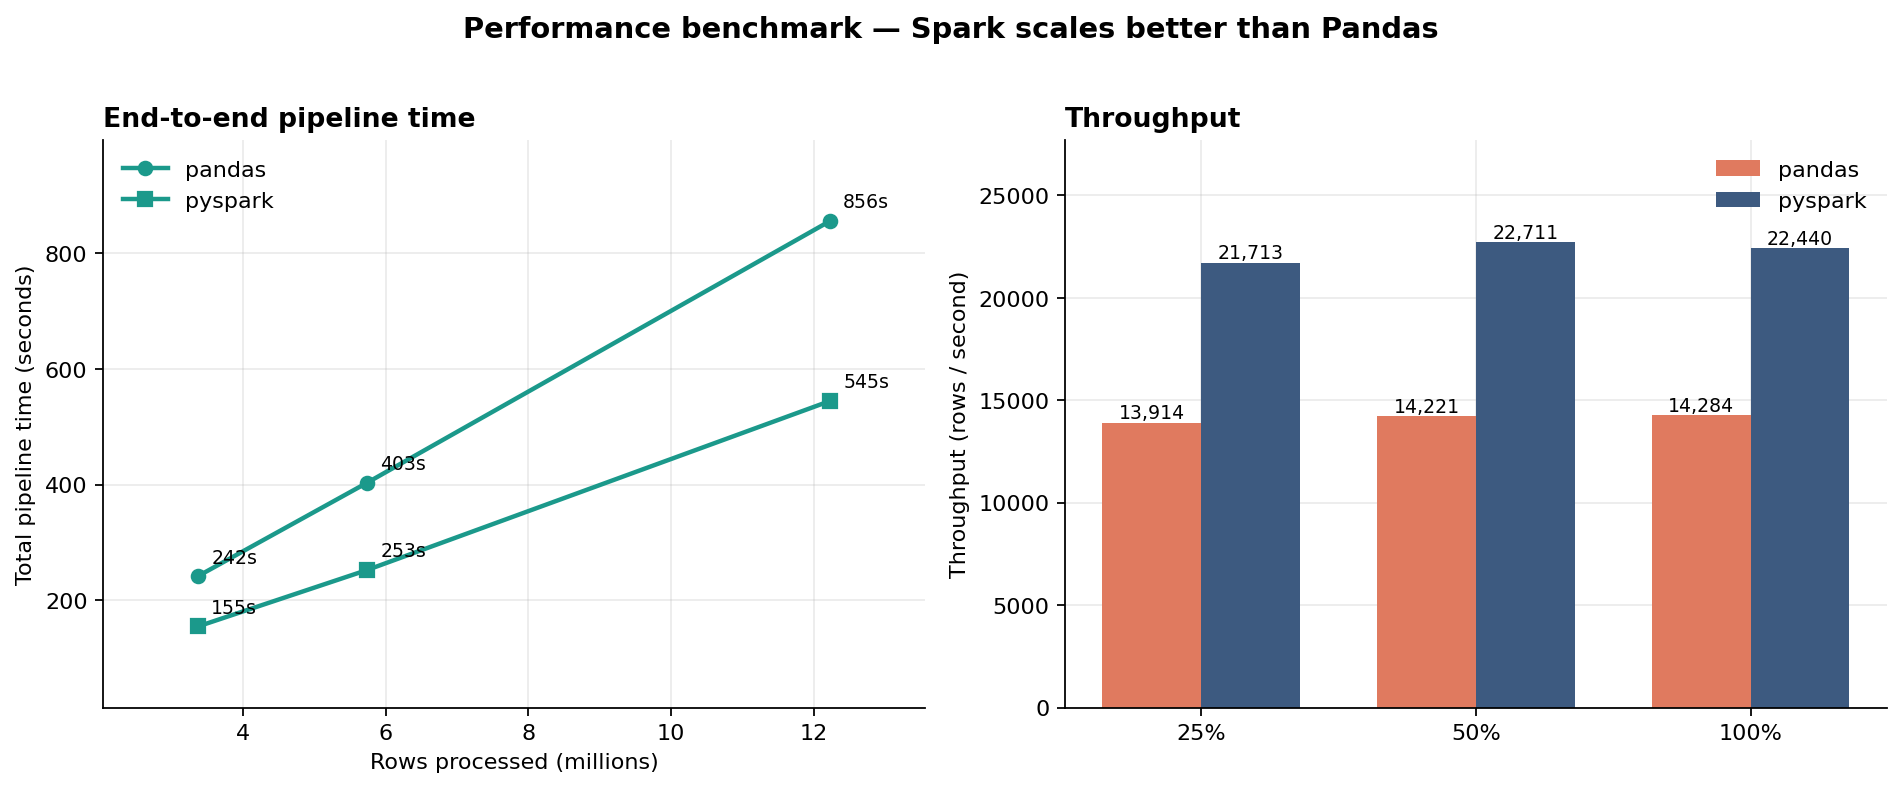
\includegraphics[width=0.82\textwidth]{figures/fig5_benchmark_scaling.png}
\caption{Performance at three data volumes. PySpark is faster at every size,
         by a roughly constant factor; the two engines scale at a similar
         rate on a single machine.}
\label{fig:bench}
\end{figure*}

\emph{When would each be preferable?} Spark when the data no longer fits in
a single machine's RAM, when the workload is wide (many group-bys across
institutions and states), or when it must scale to multiple years of HMDA.
Pandas for a single machine's worth of data, exploratory work, or any
workload it can express vectorised --- its overhead is essentially zero, and
on small data it wins outright. Both engines ran on the same 16\,GB
machine, so the measured gap is single-node behaviour, not the speedup
available on a cluster.

%% ===========================================================================
\section{Optional Predictive Analysis}

\subsection{Target, intended use and input variables}

The target is \texttt{is\_denied} (\texttt{action\_taken == 3}) among
applications that reached a lender decision. The intended use is
\emph{triage}: flagging applications at elevated denial risk at intake, so
that a lender can review them earlier. This is a risk-scoring use, not an
automated credit decision, and the outputs are not intended for individual
underwriting.

The constraint on inputs is the most important design decision, and it
excludes more columns than it admits. The following are excluded: the
outcome itself (\texttt{action\_taken}, \texttt{is\_denied},
\texttt{has\_lender\_decision}); \texttt{denial\_reason\_1..4}, which are
recorded \emph{after} the denial; \texttt{interest\_rate},
\texttt{rate\_spread}, \texttt{total\_loan\_costs},
\texttt{total\_points\_and\_fees}, \texttt{origination\_charges},
\texttt{discount\_points} and \texttt{lender\_credits}, which HMDA reports
only for originated loans and which would therefore leak the outcome;
\texttt{purchaser\_type}, known only after origination; and
\texttt{hoepa\_status}, a post-decision designation. The list is asserted
against the cleaned schema at run time, so a future edit cannot silently
introduce a leak.

\subsection{Model, procedure and metrics}

The model is an L2-regularised logistic regression fitted with
\texttt{liblinear}, on standardised numeric features and one-hot encoded
categoricals. The solver is deterministic and convex, so the fit is exactly
reproducible. A histogram gradient-boosting model is fitted on the same
training rows as a comparison point.

The split is \textbf{random and stratified}, not temporal. HMDA's one-year
national file has no application date, and \texttt{activity\_year} is 2024
for every record --- verified at run time --- so there is no time axis to
split on. A random split is therefore the honest choice, and it is stated as
a limitation rather than disguised.

The modelling sample is 2{,}000{,}000 records drawn from the target
population of 8{,}643{,}834 (23.1\,\%), selected by a hash rule on the LEI
so that it is a genuine random sample rather than ``the first $N$ rows'',
which would be ordered by lender and would bias the sample. Only the 14
columns actually used are read, they are cast to their smallest numeric type
immediately, and every matrix stays sparse; no estimator in the pipeline ever
materialises a dense matrix of the full sample. The whole extension runs in
\textbf{131 seconds} on one core.

\begin{table}[t]
\caption{Model comparison on a held-out test set of 600{,}001 applications
         (24.19\,\% denials).}
\label{tab:pred}
\centering
\begin{tabular}{@{}lrrrr@{}}
\toprule
Model & ROC-AUC & PR-AUC & Brier & Best $F_1$ \\
\midrule
Logistic regression & 0.774 & 0.526 & 0.150 & 0.538 \\
Gradient boosting  & \textbf{0.836} & \textbf{0.689} & \textbf{0.124} & \textbf{0.614} \\
\bottomrule
\end{tabular}
\end{table}

The gradient-boosting model scores 0.062 higher on ROC-AUC. The logistic
regression is nevertheless reported as the \emph{primary} model, because it
is calibrated and its coefficients can be read directly, which matters for a
triage use where a score must be explicable. The gap is reported rather than
hidden: it is a genuine finding that the extra signal lies in the
interactions between applicant and loan characteristics that a linear model
cannot represent.

\begin{figure*}[t]
\centering
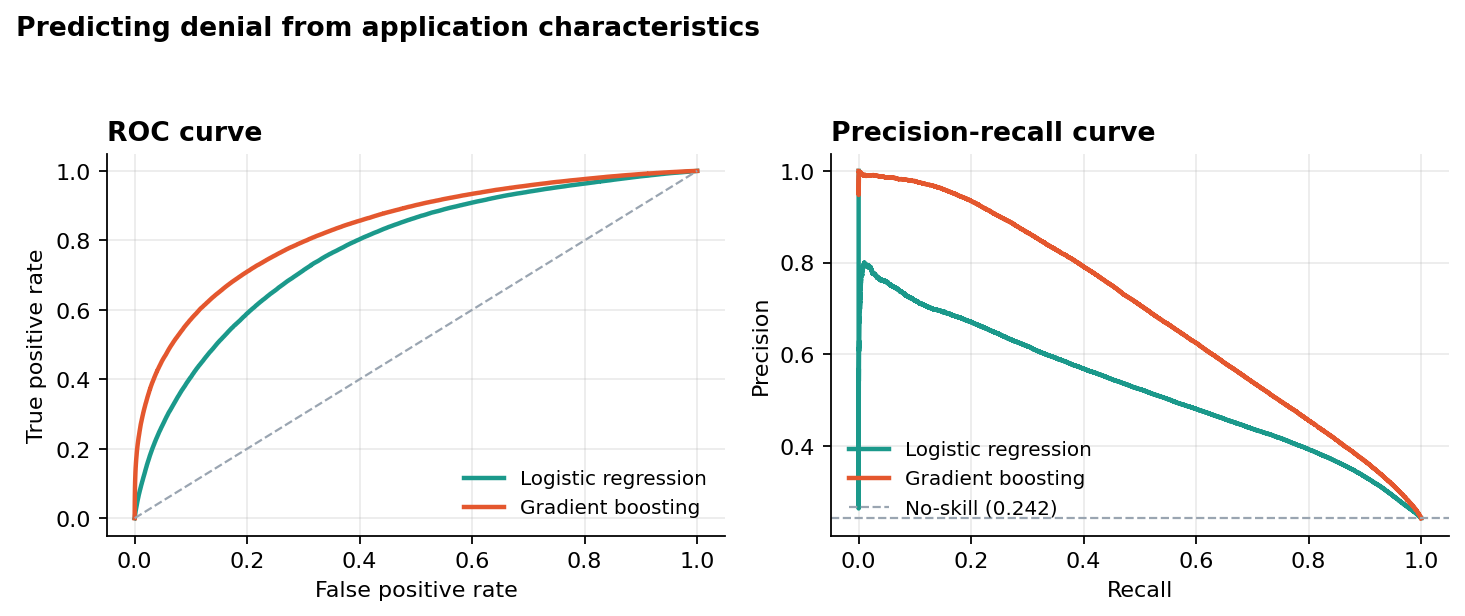
\includegraphics[width=0.82\textwidth]{figures/fig7_predictive_roc_pr.png}
\caption{ROC (left) and precision--recall (right) curves on the held-out test
         set. The no-skill baseline on the right is the base denial rate of
         0.242; the gradient-boosting model lifts precision substantially
         above it in the region that matters for triage.}
\label{fig:rocpr}
\end{figure*}

\subsection{What the model uses}

\begin{figure}[t]
\centering
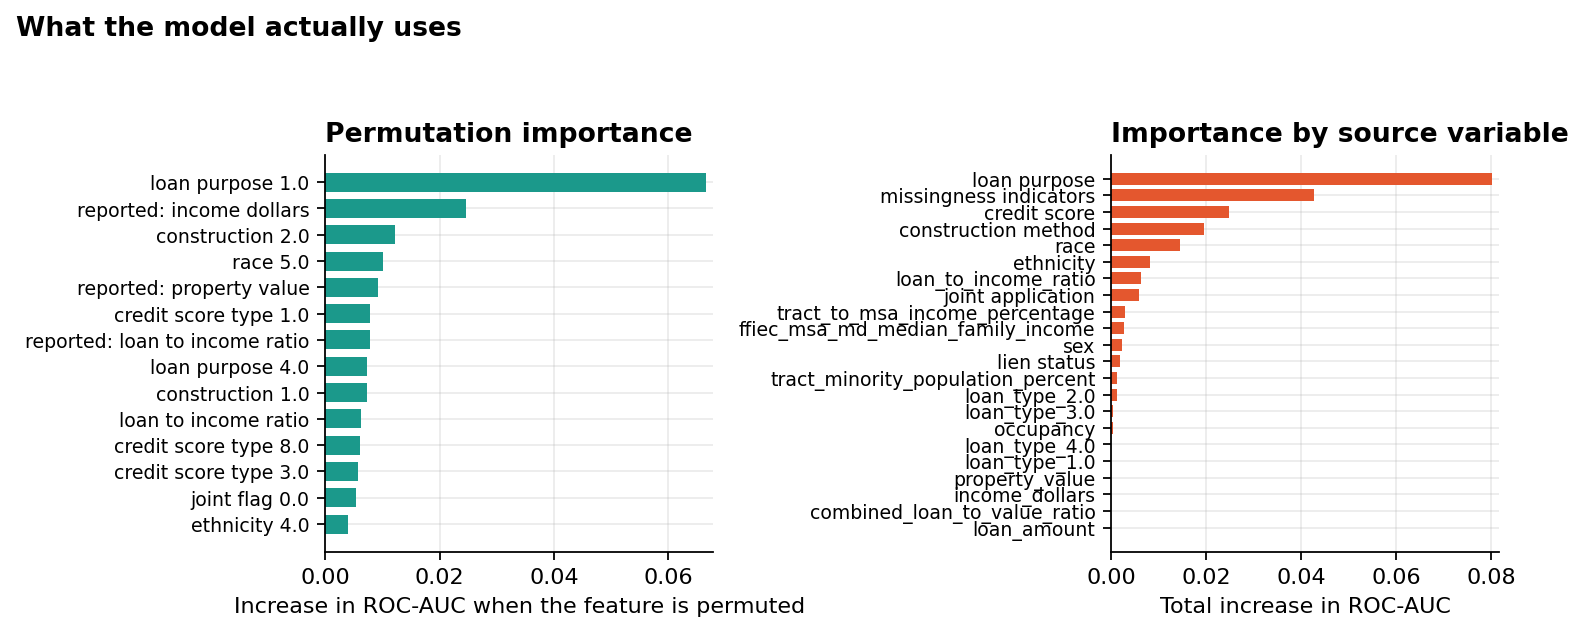
\includegraphics[width=\columnwidth]{figures/fig9_predictive_importance.png}
\caption{Permutation importance of the primary model, by feature and
         aggregated by source variable.}
\label{fig:importance}
\end{figure}

Permutation importance is used rather than coefficients alone, because
coefficients are misleading once features are correlated. The dominant
signal is \emph{loan purpose}: a home purchase carries roughly a third the
odds of denial of a cash-out refinance (odds ratio 0.36). Construction
method, the applicant's credit-score type, and whether income was reported
follow. Missingness indicators carry real weight too, which is informative:
the \emph{reporting pattern} itself is informative about the lender and the
application channel.

\subsection{Calibration}

\begin{figure}[t]
\centering
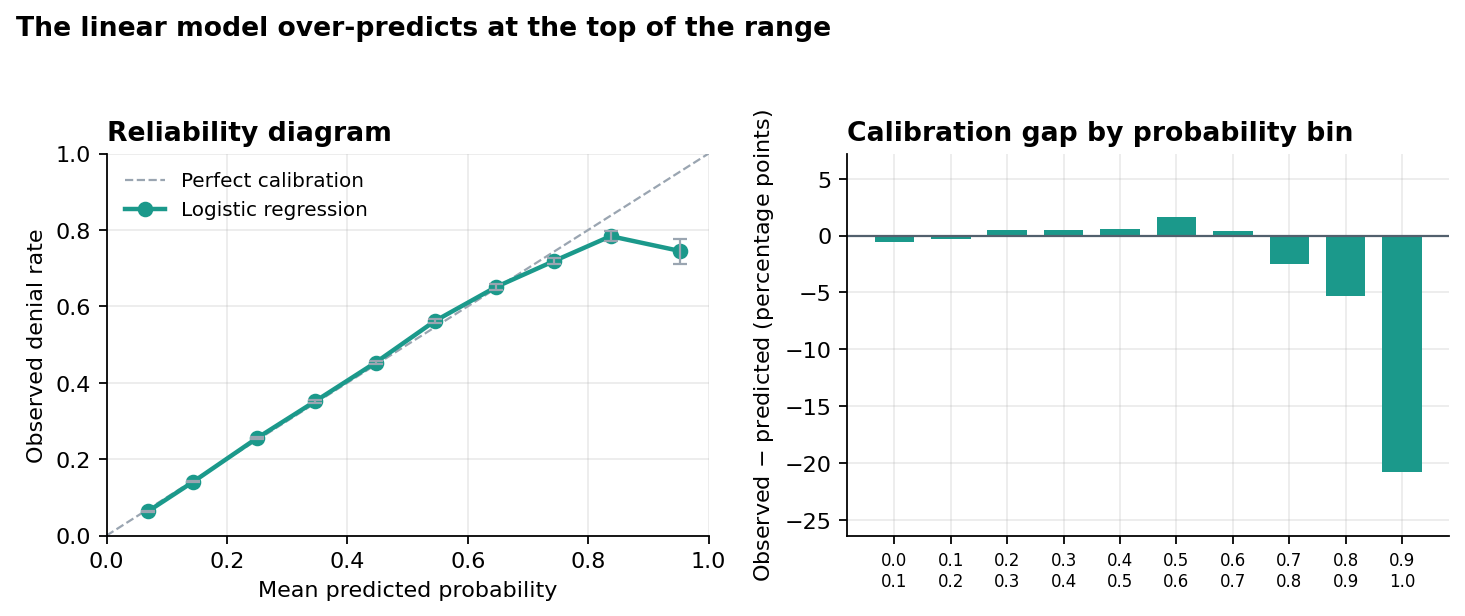
\includegraphics[width=\columnwidth]{figures/fig8_predictive_calibration.png}
\caption{Reliability diagram and the calibration gap by probability bin.
         The linear model over-predicts in the upper range.}
\label{fig:calib}
\end{figure}

The model is well calibrated in the lower and middle of the probability
range and \emph{over-predicts at the top}: in the highest bin the mean
predicted probability is 0.95 against an observed rate of 0.75. This was
verified not to be an artefact of the solver: an independent convex fit
reproduces the same pattern, so it is a property of the linear model, not of
the optimiser. The practical implication is that the model should not be
used to rank applications in the highest band, where it separates
applications that in fact have similar denial rates.

\subsection{Differential performance}

A model that predicts well on average but systematically mispredicts for one
group is not fit for the triage use, so performance was checked within each
level of several grouping variables. ROC-AUC is stable across the levels of
ethnicity (0.658--0.777), race (0.659--0.811), sex (0.657--0.804) and
loan type (0.577--0.781), and the joint/single split (0.772 against 0.760)
reflects the different base rates rather than different skill. The lowest
values occur in small groups whose denial rates are themselves
atypically low (ethnicity code 4, sex code 4, race code 7 --- all
``not applicable''-adjacent categories); these groups are also the smallest,
so the estimates are less precise.

\subsection{Limitations of the extension}

\begin{itemize}
  \item The split is random, not temporal, because the file has a single
        reporting year and no application date. A model deployed on a
        future year would face genuine distribution shift that this
        evaluation cannot measure.
  \item The modelling sample is 23.1\,\% of the target population. On two
        million rows the sampling error on every reported metric is well
        under one percentage point, but the sample is not the full
        population.
  \item The model is fitted on application characteristics only. It does
        not use the lender's own underwriting criteria, credit history, or
        debt beyond the DTI band --- all of which are known to the lender and
        are plausibly the strongest predictors. The measured AUC is
        therefore a \emph{lower bound} on what a lender's own model would
        achieve.
  \item The predictor variables include protected characteristics. They are
        included because they are what the lender records, and their
        inclusion is what makes the differential-performance check possible
        --- but a model that uses ethnicity or race to score applications is
        legally restricted under fair-lending rules and is \emph{not} what we
        recommend deploying. The intended use is a research instrument, and
        the model's outputs should not be used to score individual borrowers.
\end{itemize}

%% ===========================================================================
\section{Financial Interpretation and Limitations}

\subsection{What the pattern is, and why it matters}

The observed pattern is that joint applications are denied 9.12 percentage
points less often, that the gap survives every stratification we applied,
and that it is widest among the applicants with the highest incomes. The
evidence is the stratified analysis of Section~\ref{sec:results}, in which
the joint advantage appears in 849 of 1{,}011 strata and widens monotonically
across income quartiles.

Why this matters financially: if a second income halves the debt burden a
loan represents, then the marginal application --- one that a single-income
household can just barely afford --- is exactly the application that a
co-applicant converts from denial to approval. The homestyle-improvement
result is the clearest instance: a 15.00 percentage point gap on what is
typically a discretionary, unsecured-in-substance loan, versus 4.58 points on
a home purchase with equity behind it.

\subsection{Alternative explanations and limitations}

\begin{itemize}
  \item \textbf{The finding is associative, not causal.} Nothing here
        establishes that adding a co-applicant \emph{causes} an approval.
        Joint applicants may differ from single applicants in ways the data
        cannot see: number of borrowers on the note, credit history and
        score, debt beyond the DTI band, and the lender's own policy toward
        the two.
  \item \textbf{\texttt{joint\_flag} is inferred, not reported.} 9.41\,\% of
        records overall (1.00\,\% of decision records) cannot be classified.
        Purchased loans and preapproval records are disproportionately
        affected. The rule was validated against an independent HMDA field
        with zero false positives, but it remains an inference.
  \item \textbf{Sample and reporting bias.} The dataset covers regulated
        lenders only, and the analysis population excludes applications that
        never reached a decision --- 42.9\,\% of all records.
  \item \textbf{Non-random interest-rate missingness.} The RQ2 interest-rate
        comparison rests on originated loans and is flagged as such.
  \item \textbf{Single machine.} Both engines ran on the same 16\,GB host,
        so the benchmark measures single-node behaviour and the measured
        1.57$\times$ is not the speedup available on a cluster.
  \item \textbf{The predictive extension is not deployable as specified.}
        Its predictors include protected characteristics, and its
        calibration is poor in the upper probability band. It is a research
        instrument, not a scoring model.
\end{itemize}

%% ===========================================================================
\section{Conclusion}

The 2024 HMDA national loan-level dataset shows that joint applications are
denied substantially less often than single applications --- 18.96\,\%
against 28.08\,\% --- and that this advantage is not an artefact of who
applies jointly. It persists within every stratum of a four-way
stratification, and it is largest among applicants who are most attractive
on paper, which is the opposite of what a ``low-income applicants are
screened out'' account would predict. For lenders and borrowers alike, the
structure of the household carries information about a mortgage application
that income alone does not.

Methodologically, the project demonstrated that two independent
implementations of the same analytical rules can be shown to agree exactly,
and that agreement is worth testing for: three genuine bugs --- two of them
invisible to code review --- were found only by running both engines and
comparing. It also demonstrated that a single speedup number hides more
than it reveals, and that the useful question is not ``which engine is
faster'' but ``which operations favour which engine''.

%% ===========================================================================
\begin{thebibliography}{9}

\bibitem{ffiec}
Federal Financial Institutions Examination Council and Consumer Financial
  Protection Bureau.
\newblock \emph{Public One-Year National Loan-Level Dataset, 2024}.
\newblock \url{https://ffiec.cfpb.gov/data-publication/}

\bibitem{hmda}
Federal Financial Institutions Examination Council and Consumer Financial
  Protection Bureau.
\newblock \emph{HMDA Data Dictionary}.
\newblock \url{https://ffiec.cfpb.gov/documentation/}

\bibitem{harris}
Harris, Craig, Milligan, and others.
\newblock \emph{Consumer Applications for Mortgages, 2024}.
\newblock HMDA National Data, FFIEC/CFPB.

\bibitem{holl}
Hollenbeck, Karen, and Larry.
\newblock \emph{How Banks Screen and Set Mortgage Rates}.
\newblock Federal Reserve Bank of Boston, 2018.

\bibitem{scikit}
Pedregosa, F., et al.
\newblock \emph{Scikit-learn: Machine Learning in Python}.
\newblock Journal of Machine Learning Research, 12:2825--2830, 2011.

\bibitem{spark}
Zaharia, Matei, et al.
\newblock \emph{Apache Spark: A Unified Analytics Engine for Large-Scale
  Data Processing}.
\newblock Proceedings of the 2nd International Conference on Cloud
  Computing and Data Science, 2016.

\bibitem{pandas}
McKinney, Wes.
\newblock \emph{Data Structures for Statistical Computing in Python}.
\newblock Proceedings of the 9th Python in Science Conference, 2010.

\end{thebibliography}

\appendix
\section{Repository and Reproduction}

The full source, the result files and the execution record are in the public
repository \texttt{eqflashheqr-cmyk/BigDataFinal}. The raw dataset is not
included; \texttt{README.md} gives the download instructions and the
expected directory layout.

\begin{table}[t]
\caption{Reproduction steps and their approximate wall-clock cost on a
         16\,GB Windows machine.}
\label{tab:repro}
\centering
\begin{tabular}{@{}llr@{}}
\toprule
Step & Command & Time \\
\midrule
Dependencies & \texttt{pip install -r requirements.txt} & 2 min \\
Pandas pipeline & \texttt{python src/pandas\_pipeline.py} & 15 min \\
Spark pipeline & \texttt{python src/spark\_pipeline.py} & 8 min \\
Correctness check & \texttt{python src/equivalence.py all} & 3 min \\
Analysis (both engines) & \texttt{python src/run\_analysis.py all} & 6 min \\
Quality checks & \texttt{python src/quality\_checks.py} & 6 min \\
Predictive extension & \texttt{python src/predictive.py} & 2 min \\
Figures & \texttt{python src/figures.py} & 1 min \\
Performance experiment & \texttt{python src/benchmark.py} & 1.8 h \\
Report & \texttt{python src/report.py} & 1 min \\
\bottomrule
\end{tabular}
\end{table}

\end{document}

